% TEMPLATE for Usenix papers, specifically to meet requirements of
%  USENIX '05
% originally a template for producing IEEE-format articles using LaTeX.
%   written by Matthew Ward, CS Department, Worcester Polytechnic Institute.
% adapted by David Beazley for his excellent SWIG paper in Proceedings,
%   Tcl 96
% turned into a smartass generic template by De Clarke, with thanks to
%   both the above pioneers
% use at your own risk.  Complaints to /dev/null.
% make it two column with no page numbering, default is 10 point

% Munged by Fred Douglis <douglis@research.att.com> 10/97 to separate
% the .sty file from the LaTeX source template, so that people can
% more easily include the .sty file into an existing document.  Also
% changed to more closely follow the style guidelines as represented
% by the Word sample file. 

% Note that since 2010, USENIX does not require endnotes. If you want
% foot of page notes, don't include the endnotes package in the 
% usepackage command, below.

% This version uses the latex2e styles, not the very ancient 2.09 stuff.
\documentclass[letterpaper,twocolumn,10pt]{article}


\usepackage{usenix,epsfig,endnotes}
\usepackage{amsmath}
\usepackage{mathtools,xparse}
\usepackage{graphicx}


\newcommand{\bibsc}[1]{{\sc#1}}
\newcommand{\bibemph}[1]{{\em#1}}
\newcommand{\bibemphic}[1]{{\em#1\/}}
\newcommand{\bibyear}[2]{%
\unskip\quad\ignorespaces#1\unskip
\if#2. .\quad \else \quad#2 \fi
}

\DeclarePairedDelimiter{\abs}{\lvert}{\rvert}
\DeclarePairedDelimiter{\norm}{\lVert}{\rVert}


\begin{document}

%don't want date printed
\date{}

%make title bold and 14 pt font (Latex default is non-bold, 16 pt)
\title{\Large \bf Recommender Systems for NYC Residential Community}

%for single author (just remove % characters)
\author{
{\rm Nicholas Souris}\\
ns3205@nyu.edu
\and
{\rm Yanhong Yang}\\
yy1553@nyu.edu
% copy the following lines to add more authors
 \and
 {\rm Zeleng Zhuang}\\
zz1135@nyu.edu
} % end author

\maketitle

% Use the following at camera-ready time to suppress page numbers.
% Comment it out when you first submit the paper for review.
\thispagestyle{empty}


\subsection*{Abstract}
In this paper we will  present the process and algorithms that are used into creating a house recommender system for residences situated in the area of the city of New York. The algorithms used, will be compared and contrasted or even merged (thus creating new hybrid recommender algorithms) in an effort to magnify the accuracy of our system. The resulting data outputs from the usage and application of recommender algorithms, will be cleansed, indexed and filtered in such a way that the feasibility of a final merge, in an effort to converge to a single or a small group of accurate recommendations for a suitable residence, will almost be assured.


\section{Introduction}

Finding an apartment to rent or buy in New York city can be a daunting task and can very well become a source of  deep frustration. Defining a suitable place of residence is a completely subjective matter which mostly has to do with the buyer's or renter's preferences. Living in an area with low crime rate or amongst a local populace with a specific affinity in regards to traditional family values or even in close proximity to high ranking restaurants can be some of the reasons why a person would choose  to live in a certain area over another. Coupling the vast amount of information required to choose where to live with the high housing prices and large area diversity  of a metropolitan area such as New York city, it is fairly easy to recognize how recommending a specific house to a potential buyer or renter can become a disheartening job. 

Our project aims to use historical data regarding housing prices along with several other parameters that might affect the standard of living of residents, in an effort to create a recommender system for NYC residential communities based on zip code. 

We will collect data including housing prices, income, safety, infrastructure and other commonly used factors in evaluating a residential community. We will attempt to discover all or most of the necessary techniques which are vital for the practical implementation of a housing recommender system. Given that  the timeframe in which we need to implement this system is large enough, a platform will be built for the recommender system for the purpose of collecting data from anonymous volunteer users that are willing to provide information to enrich our database.
In this paper, the motivation, research and the thought processes that led to the final design will become transparent and brought to the foreground in an effort to substantiate the accuracy and efficacy of our analytics project.


%\section{Motivation}
%(Write a couple of paragraphs describing why you think this analytic is important. Why should people care about this analytic?)
%

\section{Related Work}
There are three main categories of recommendation methods:  content-based, collaborative, and hybrid recommendation approaches. 
 Content-based systems recommend items similar to the ones that a user preferred in the past,  collaborative systems recommend items  that people with similar tastes and preferences liked in the past, while  hybrid recommender systems by combining collaborative and content-based methods  can avoid certain limitations of content-based and collaborative systems. \cite{AT05} has presented an overview of the field of recommender systems.
 
 In content-based recommendation methods, the utility $u(c, s)$ of item $s$  for user $c$ is estimated based on $u(c, s_i)$ where items $s_i$ are ``similar'' to $s$ and usually defined as:
 \begin{align*}
  u(c, s) = \text{score}(ContentBasedProfile(c), Content(s)),
  \end{align*}
 where $ ContentBasedProfile(c)$ is the profile of user $c$ containing tastes and preferences of this user,  and $ Content(s)$ is an item profile consisting of attributes characterizing item $s$. 
 In information retrieval-based paradigm of recommending Web pages, Web site URLs or news messages, both $ ContentBasedProfile(c)$ and $ Content(s)$ can be represented as \textit{term frequency/inverse document frequency} \cite{S89}  (TF-IDF) vectors $\overrightarrow{\omega}_c$ and $\overrightarrow{\omega}_s$ of keyword weight; and utility function $u(c, s)$ is represented as the cosine similarity measure \cite{BYRN99}, \cite{S89}:
\begin{align}
 u(c, s) = \cos(\overrightarrow{\omega}_c, \overrightarrow{\omega}_s) = \frac{\overrightarrow{\omega}_c\cdot \overrightarrow{\omega}_s}{\norm{\overrightarrow{\omega}_c}_2\times \norm{\overrightarrow{\omega}_s}_2}.
 \end{align}



In collaborative filtering systems, the utility function $u(c, s)$ of item $s$ for user $c$ is estimated based on $u(c_j, s)$ of item $s$ for users $c_j$ who are ``similar" to $c$.
Various algorithms have been developed to make rating predictions, in general grouped into two classes  \cite{BHK98}:  \textit{memory-based} (or \textit{heuristic-based}) and \textit{model-based}.
For memory-based algorithms, the value of an unknown rating $r_{c,s}$ for user $c$ and item $s$ is usually computed as an aggregate function of the ratings $r_{c',s}$   of the most $N$ similar users to $c$ for the same item $s$. A lot of approaches have been applied to compute the similarity $sim(c, c') $ between two users, most of which are based on their ratings of items that both users have rated; the two most popular approaches are correlation and cosine-based.  The Pearson correlation coefficient  used to measure similarity  is defined as follows \cite{RISBR94}, \cite{SM95}:
\begin{align}
 sim(c, c') = \frac{ (\gamma_c-\overline{\gamma}_{c}) \cdot (\gamma_{c'}-\overline{\gamma}_{c'}) }{\norm{\gamma_c-\overline{\gamma}_{c}}_2\times \norm{\gamma_{c'}-\overline{\gamma}_{c'}}_2}.\end{align}

Besides the heuristic rules,  statistical and machine learning techniques have also  been applied to  learn a model. For example, \cite{BHK98} proposes a probabilistic approach calculate the unknown ratings:
\begin{align} \label{prob}
r_{c, s} = E(r_{c, s}) = \sum_{i=0}^n i\times \text{Pr}(r_{c, s} =i\ |\ r_{c, s'}, s'\in S_c ), 
\end{align}
where rating values are assumed to be integers between  0 and $n$ and the probability expression is the probability that user $c$ will give a particular rating to item $s$ given user $c$'s ratings of previously rated items $S_c$.  In order to estimate  the probability, \cite{BHK98} also proposes two  probabilistic models: cluster model and Bayesian networks.  

In \cite{AT05}, the methods of combining  collaborative and content-based systems are classified into four classes:
\begin{enumerate}
\item implementing collaborative and content-based methods separately, and combining their predictions;
\item incorporating content-based characteristics into a collaborative approach;
\item incorporating collaborative characteristics into a content-based approach;
\item constructing a general unifying model that incorporates both content-based and collaborative characteristics.
\end{enumerate}

Moreover, \cite{AT05}  describes various limitations of current recommendation methods and discusses possible extensions that can improve recommendation capabilities. 

\section{Design}
See Figure 1.

\begin{figure}[h!]\label{fig1}
\begin{center}
%\begin{picture}(400,150)(100,200)
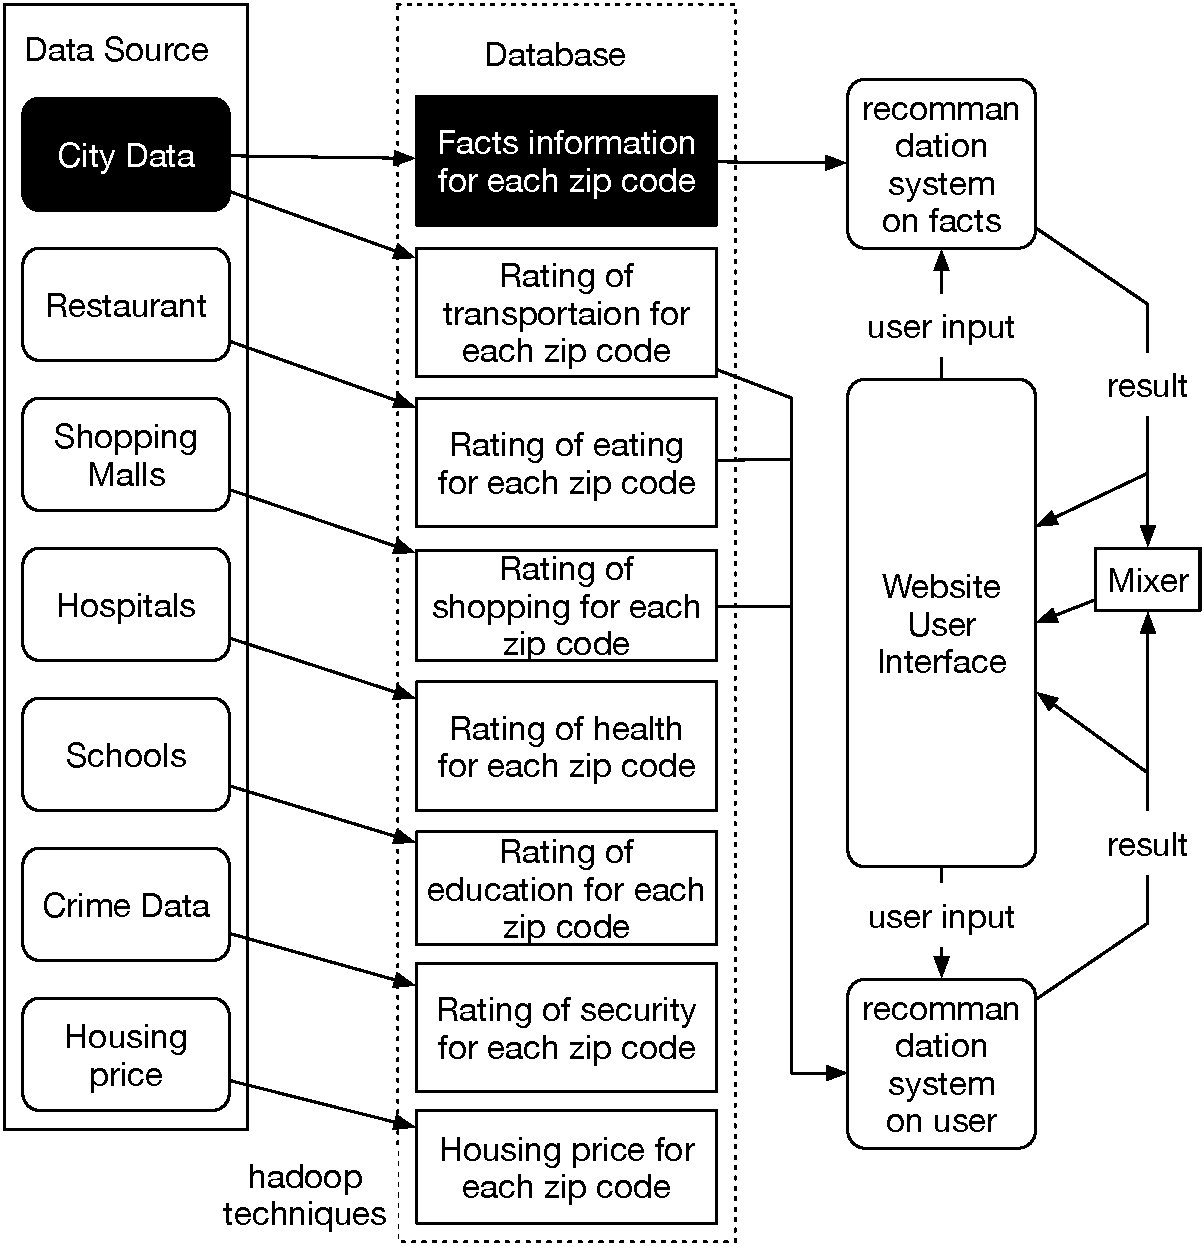
\includegraphics[width=0.5\textwidth]{design.pdf}
%\put(-15,-30){\special{psfile = fig1.ps hscale = 50 vscale = 50}}
%\end{picture}\\
\end{center}
\caption{ Design of Recommender System}
\end{figure}

\section{Results}
(Future? In this section, you can describe: Your experimental setup/issues with data/performance/etc. Describe your experiments, describe what you learned. Did you prove or disprove your hypothesis? Were some results unexpected? Why? )

\section{Future Work}
(Future? Given time, how would you expand your analytic? Could it be applied to other areas? Etc?)

\section{Conclusion}
(Future? One or two paragraphs about the value/accuracy/goodness of your analytic.)



%\section{This Section has SubSections}
%\subsection{First SubSection}
%
%Here's a typical figure reference.  The figure is centered at the
%top of the column.  It's scaled.  It's explicitly placed.  You'll
%have to tweak the numbers to get what you want.\\
%
%% you can also use the wonderful epsfig package...
%\begin{figure}[t]
%\begin{center}
%\begin{picture}(300,150)(0,200)
%\put(-15,-30){\special{psfile = fig1.ps hscale = 50 vscale = 50}}
%\end{picture}\\
%\end{center}
%\caption{Wonderful Flowchart}
%\end{figure}
%
%This text came after the figure, so we'll casually refer to Figure 1
%as we go on our merry way.
%
%\subsection{New Subsection}
%
%It can get tricky typesetting Tcl and C code in LaTeX because they share
%a lot of mystical feelings about certain magic characters.  You
%will have to do a lot of escaping to typeset curly braces and percent
%signs, for example, like this:
%``The {\tt \%module} directive
%sets the name of the initialization function.  This is optional, but is
%recommended if building a Tcl 7.5 module.
%Everything inside the {\tt \%\{, \%\}}
%block is copied directly into the output. allowing the inclusion of
%header files and additional C code." \\
%
%Sometimes you want to really call attention to a piece of text.  You
%can center it in the column like this:
%\begin{center}
%{\tt \_1008e614\_Vector\_p}
%\end{center}
%and people will really notice it.\\
%
%\noindent
%The noindent at the start of this paragraph makes it clear that it's
%a continuation of the preceding text, not a new para in its own right.
%
%
%Now this is an ingenious way to get a forced space.
%{\tt Real~$*$} and {\tt double~$*$} are equivalent. 
%
%Now here is another way to call attention to a line of code, but instead
%of centering it, we noindent and bold it.\\
%
%\noindent
%{\bf \tt size\_t : fread ptr size nobj stream } \\
%
%And here we have made an indented para like a definition tag (dt)
%in HTML.  You don't need a surrounding list macro pair.
%\begin{itemize}
%\item[]  {\tt fread} reads from {\tt stream} into the array {\tt ptr} at
%most {\tt nobj} objects of size {\tt size}.   {\tt fread} returns
%the number of objects read. 
%\end{itemize}
%This concludes the definitions tag.
%
%\subsection{How to Build Your Paper}
%
%You have to run {\tt latex} once to prepare your references for
%munging.  Then run {\tt bibtex} to build your bibliography metadata.
%Then run {\tt latex} twice to ensure all references have been resolved.
%If your source file is called {\tt usenixTemplate.tex} and your {\tt
% bibtex} file is called {\tt usenixTemplate.bib}, here's what you do:
%{\tt \small
%\begin{verbatim}
%latex usenixTemplate
%bibtex usenixTemplate
%latex usenixTemplate
%latex usenixTemplate
%\end{verbatim}
%}
%
%
%\subsection{Last SubSection}
%
%Well, it's getting boring isn't it.  This is the last subsection
%before we wrap it up.

\section{Acknowledgments}

(This section is optional. It can be used to thank the  people/companies/organizations who have made data available to you, for example. You can list any HPC people who were particularly helpful, if you used the NYU HPC.)


 
 
{\footnotesize \bibliographystyle{acm}
%\bibliography{../common/bibliography}}
  \begin{thebibliography}{}
  
\bibitem{AT05} \bibsc{G. Adomavicius and A. Tuzhilin.} Toward the Next Generation of Recommender Systems: A Survey of the State-of-the-Art and Possible Extensions. \bibemphic{IEEE Trans. Knowl. Data Eng.} \bibemph{17}, 6 (June 2005), pp. 734--749
  
  \bibitem{BYRN99} \bibsc{R. Baeza-Yates and B. Ribeiro-Neto.} \bibemph{Modern information Retrieval.} Addison-Wesley, 1999.
  
  \bibitem{BHK98} \bibsc{ J.S. Breese, D. Heckerman and C.Kadie.}  \bibemph{Empirical Analysis of Predictive Algorithms for Collaborative Filtering.} In Proc. 14th Conf. Uncertainty in Artificial Intelligence, July 1998. 
  
  \bibitem{DG04} \bibsc{ J. Dean and S. Ghemawat.}  \bibemph{MapReduce: Simplified data processing on large clusters.} In proceedings of 6th Symposium on Operating Systems Design and Implemenation, 2004.
  
  \bibitem{G11} \bibsc{A. Gates.} \bibemph{Programming Pig.} O?Reilly Media Inc., Sebastopol, CA,  October 2011.
  
  \bibitem{GGL03} \bibsc{ S. Ghemawat, H. Gobioff and S. T. Leung.} \bibemph{The Google File System.}
  In Proceedings of the nineteenth ACM Symposium on Operating Systems Principles -- SOSP `03, 2003.
  
  
  \bibitem{PB07}
  \bibsc{M. J. Pazzani and  D. Billsus.}  \newblock Content-based recommendation systems.  IN P. Brusilovsky, A. Kobsa, and W. Nejdl (Eds.):  \bibemphic{ The adaptive web,} LNCS. 4321, pp. 325--341, 2007. 
  
  \bibitem{RISBR94} \bibsc{P. Resnick, N. Iakovou, M. Sushak, P. Bergstrom, and J. Riedl.} \bibemph{GroupLens: An Open Architecture for Collaborative Filtering of Netnews.} In Proc. Computer Supported Cooperative Work Conf., 1994.
  
  
  \bibitem{S89} \bibsc{G. Salton.} \bibemph{Automatic Text Processing.} Addison-Wesley, 1989.
 
 \bibitem{SM95} \bibsc{U. Shardanand and P. Maes.} \bibemph{Social Information Filtering: Algorithms for Automating ``Word of Mouth".} In Proc. Conf. Human Factors in Computing Systems, 1995. 
 
  \bibitem{W12} \bibsc{T. White.} \bibemph{Hadoop: The Definitive Guide.} O?Reilly Media Inc., Sebastopol, CA, May 2012.
%
%   \bibitem{salas:calculus}
% %  \protect\citeauthoryear{Salas and Hille}{Salas and Hille}{1978}
%\bibsc{Salas, S. and Hille, E.}
%\bibemph{Calculus: One and Several Variable}.
%John Wiley and Sons, New York.  \bibyear{1978}.
%
%\bibitem{herlihy:methodology}
%%\protect\citeauthoryear{Herlihy}{Herlihy}{1993}
%\bibsc{Herlihy, M.} 
%\newblock A methodology for implementing highly concurrent data objects.
% \bibemphic{ACM Trans. Program. Lang. Syst.} ~\bibemph{15}, 5 (November 1993), 745--770. 
%
  
   \end{thebibliography}


%\theendnotes

\end{document}






